
% Default to the notebook output style

    


% Inherit from the specified cell style.




    
\documentclass{article}

    
    
    \usepackage{graphicx} % Used to insert images
    \usepackage{adjustbox} % Used to constrain images to a maximum size 
    \usepackage{color} % Allow colors to be defined
    \usepackage{enumerate} % Needed for markdown enumerations to work
    \usepackage{geometry} % Used to adjust the document margins
    \usepackage{amsmath} % Equations
    \usepackage{amssymb} % Equations
    \usepackage[mathletters]{ucs} % Extended unicode (utf-8) support
    \usepackage[utf8x]{inputenc} % Allow utf-8 characters in the tex document
    \usepackage{fancyvrb} % verbatim replacement that allows latex
    \usepackage{grffile} % extends the file name processing of package graphics 
                         % to support a larger range 
    % The hyperref package gives us a pdf with properly built
    % internal navigation ('pdf bookmarks' for the table of contents,
    % internal cross-reference links, web links for URLs, etc.)
    \usepackage{hyperref}
    \usepackage{longtable} % longtable support required by pandoc >1.10
    \usepackage{booktabs}  % table support for pandoc > 1.12.2
    

    
    
    \definecolor{orange}{cmyk}{0,0.4,0.8,0.2}
    \definecolor{darkorange}{rgb}{.71,0.21,0.01}
    \definecolor{darkgreen}{rgb}{.12,.54,.11}
    \definecolor{myteal}{rgb}{.26, .44, .56}
    \definecolor{gray}{gray}{0.45}
    \definecolor{lightgray}{gray}{.95}
    \definecolor{mediumgray}{gray}{.8}
    \definecolor{inputbackground}{rgb}{.95, .95, .85}
    \definecolor{outputbackground}{rgb}{.95, .95, .95}
    \definecolor{traceback}{rgb}{1, .95, .95}
    % ansi colors
    \definecolor{red}{rgb}{.6,0,0}
    \definecolor{green}{rgb}{0,.65,0}
    \definecolor{brown}{rgb}{0.6,0.6,0}
    \definecolor{blue}{rgb}{0,.145,.698}
    \definecolor{purple}{rgb}{.698,.145,.698}
    \definecolor{cyan}{rgb}{0,.698,.698}
    \definecolor{lightgray}{gray}{0.5}
    
    % bright ansi colors
    \definecolor{darkgray}{gray}{0.25}
    \definecolor{lightred}{rgb}{1.0,0.39,0.28}
    \definecolor{lightgreen}{rgb}{0.48,0.99,0.0}
    \definecolor{lightblue}{rgb}{0.53,0.81,0.92}
    \definecolor{lightpurple}{rgb}{0.87,0.63,0.87}
    \definecolor{lightcyan}{rgb}{0.5,1.0,0.83}
    
    % commands and environments needed by pandoc snippets
    % extracted from the output of `pandoc -s`
    \DefineVerbatimEnvironment{Highlighting}{Verbatim}{commandchars=\\\{\}}
    % Add ',fontsize=\small' for more characters per line
    \newenvironment{Shaded}{}{}
    \newcommand{\KeywordTok}[1]{\textcolor[rgb]{0.00,0.44,0.13}{\textbf{{#1}}}}
    \newcommand{\DataTypeTok}[1]{\textcolor[rgb]{0.56,0.13,0.00}{{#1}}}
    \newcommand{\DecValTok}[1]{\textcolor[rgb]{0.25,0.63,0.44}{{#1}}}
    \newcommand{\BaseNTok}[1]{\textcolor[rgb]{0.25,0.63,0.44}{{#1}}}
    \newcommand{\FloatTok}[1]{\textcolor[rgb]{0.25,0.63,0.44}{{#1}}}
    \newcommand{\CharTok}[1]{\textcolor[rgb]{0.25,0.44,0.63}{{#1}}}
    \newcommand{\StringTok}[1]{\textcolor[rgb]{0.25,0.44,0.63}{{#1}}}
    \newcommand{\CommentTok}[1]{\textcolor[rgb]{0.38,0.63,0.69}{\textit{{#1}}}}
    \newcommand{\OtherTok}[1]{\textcolor[rgb]{0.00,0.44,0.13}{{#1}}}
    \newcommand{\AlertTok}[1]{\textcolor[rgb]{1.00,0.00,0.00}{\textbf{{#1}}}}
    \newcommand{\FunctionTok}[1]{\textcolor[rgb]{0.02,0.16,0.49}{{#1}}}
    \newcommand{\RegionMarkerTok}[1]{{#1}}
    \newcommand{\ErrorTok}[1]{\textcolor[rgb]{1.00,0.00,0.00}{\textbf{{#1}}}}
    \newcommand{\NormalTok}[1]{{#1}}
    
    % Define a nice break command that doesn't care if a line doesn't already
    % exist.
    \def\br{\hspace*{\fill} \\* }
    % Math Jax compatability definitions
    \def\gt{>}
    \def\lt{<}
    % Document parameters
    \title{03.1\_Distributed\_Computing}
    
    
    

    % Pygments definitions
    
\makeatletter
\def\PY@reset{\let\PY@it=\relax \let\PY@bf=\relax%
    \let\PY@ul=\relax \let\PY@tc=\relax%
    \let\PY@bc=\relax \let\PY@ff=\relax}
\def\PY@tok#1{\csname PY@tok@#1\endcsname}
\def\PY@toks#1+{\ifx\relax#1\empty\else%
    \PY@tok{#1}\expandafter\PY@toks\fi}
\def\PY@do#1{\PY@bc{\PY@tc{\PY@ul{%
    \PY@it{\PY@bf{\PY@ff{#1}}}}}}}
\def\PY#1#2{\PY@reset\PY@toks#1+\relax+\PY@do{#2}}

\expandafter\def\csname PY@tok@gd\endcsname{\def\PY@tc##1{\textcolor[rgb]{0.63,0.00,0.00}{##1}}}
\expandafter\def\csname PY@tok@gu\endcsname{\let\PY@bf=\textbf\def\PY@tc##1{\textcolor[rgb]{0.50,0.00,0.50}{##1}}}
\expandafter\def\csname PY@tok@gt\endcsname{\def\PY@tc##1{\textcolor[rgb]{0.00,0.27,0.87}{##1}}}
\expandafter\def\csname PY@tok@gs\endcsname{\let\PY@bf=\textbf}
\expandafter\def\csname PY@tok@gr\endcsname{\def\PY@tc##1{\textcolor[rgb]{1.00,0.00,0.00}{##1}}}
\expandafter\def\csname PY@tok@cm\endcsname{\let\PY@it=\textit\def\PY@tc##1{\textcolor[rgb]{0.25,0.50,0.50}{##1}}}
\expandafter\def\csname PY@tok@vg\endcsname{\def\PY@tc##1{\textcolor[rgb]{0.10,0.09,0.49}{##1}}}
\expandafter\def\csname PY@tok@m\endcsname{\def\PY@tc##1{\textcolor[rgb]{0.40,0.40,0.40}{##1}}}
\expandafter\def\csname PY@tok@mh\endcsname{\def\PY@tc##1{\textcolor[rgb]{0.40,0.40,0.40}{##1}}}
\expandafter\def\csname PY@tok@go\endcsname{\def\PY@tc##1{\textcolor[rgb]{0.53,0.53,0.53}{##1}}}
\expandafter\def\csname PY@tok@ge\endcsname{\let\PY@it=\textit}
\expandafter\def\csname PY@tok@vc\endcsname{\def\PY@tc##1{\textcolor[rgb]{0.10,0.09,0.49}{##1}}}
\expandafter\def\csname PY@tok@il\endcsname{\def\PY@tc##1{\textcolor[rgb]{0.40,0.40,0.40}{##1}}}
\expandafter\def\csname PY@tok@cs\endcsname{\let\PY@it=\textit\def\PY@tc##1{\textcolor[rgb]{0.25,0.50,0.50}{##1}}}
\expandafter\def\csname PY@tok@cp\endcsname{\def\PY@tc##1{\textcolor[rgb]{0.74,0.48,0.00}{##1}}}
\expandafter\def\csname PY@tok@gi\endcsname{\def\PY@tc##1{\textcolor[rgb]{0.00,0.63,0.00}{##1}}}
\expandafter\def\csname PY@tok@gh\endcsname{\let\PY@bf=\textbf\def\PY@tc##1{\textcolor[rgb]{0.00,0.00,0.50}{##1}}}
\expandafter\def\csname PY@tok@ni\endcsname{\let\PY@bf=\textbf\def\PY@tc##1{\textcolor[rgb]{0.60,0.60,0.60}{##1}}}
\expandafter\def\csname PY@tok@nl\endcsname{\def\PY@tc##1{\textcolor[rgb]{0.63,0.63,0.00}{##1}}}
\expandafter\def\csname PY@tok@nn\endcsname{\let\PY@bf=\textbf\def\PY@tc##1{\textcolor[rgb]{0.00,0.00,1.00}{##1}}}
\expandafter\def\csname PY@tok@no\endcsname{\def\PY@tc##1{\textcolor[rgb]{0.53,0.00,0.00}{##1}}}
\expandafter\def\csname PY@tok@na\endcsname{\def\PY@tc##1{\textcolor[rgb]{0.49,0.56,0.16}{##1}}}
\expandafter\def\csname PY@tok@nb\endcsname{\def\PY@tc##1{\textcolor[rgb]{0.00,0.50,0.00}{##1}}}
\expandafter\def\csname PY@tok@nc\endcsname{\let\PY@bf=\textbf\def\PY@tc##1{\textcolor[rgb]{0.00,0.00,1.00}{##1}}}
\expandafter\def\csname PY@tok@nd\endcsname{\def\PY@tc##1{\textcolor[rgb]{0.67,0.13,1.00}{##1}}}
\expandafter\def\csname PY@tok@ne\endcsname{\let\PY@bf=\textbf\def\PY@tc##1{\textcolor[rgb]{0.82,0.25,0.23}{##1}}}
\expandafter\def\csname PY@tok@nf\endcsname{\def\PY@tc##1{\textcolor[rgb]{0.00,0.00,1.00}{##1}}}
\expandafter\def\csname PY@tok@si\endcsname{\let\PY@bf=\textbf\def\PY@tc##1{\textcolor[rgb]{0.73,0.40,0.53}{##1}}}
\expandafter\def\csname PY@tok@s2\endcsname{\def\PY@tc##1{\textcolor[rgb]{0.73,0.13,0.13}{##1}}}
\expandafter\def\csname PY@tok@vi\endcsname{\def\PY@tc##1{\textcolor[rgb]{0.10,0.09,0.49}{##1}}}
\expandafter\def\csname PY@tok@nt\endcsname{\let\PY@bf=\textbf\def\PY@tc##1{\textcolor[rgb]{0.00,0.50,0.00}{##1}}}
\expandafter\def\csname PY@tok@nv\endcsname{\def\PY@tc##1{\textcolor[rgb]{0.10,0.09,0.49}{##1}}}
\expandafter\def\csname PY@tok@s1\endcsname{\def\PY@tc##1{\textcolor[rgb]{0.73,0.13,0.13}{##1}}}
\expandafter\def\csname PY@tok@sh\endcsname{\def\PY@tc##1{\textcolor[rgb]{0.73,0.13,0.13}{##1}}}
\expandafter\def\csname PY@tok@sc\endcsname{\def\PY@tc##1{\textcolor[rgb]{0.73,0.13,0.13}{##1}}}
\expandafter\def\csname PY@tok@sx\endcsname{\def\PY@tc##1{\textcolor[rgb]{0.00,0.50,0.00}{##1}}}
\expandafter\def\csname PY@tok@bp\endcsname{\def\PY@tc##1{\textcolor[rgb]{0.00,0.50,0.00}{##1}}}
\expandafter\def\csname PY@tok@c1\endcsname{\let\PY@it=\textit\def\PY@tc##1{\textcolor[rgb]{0.25,0.50,0.50}{##1}}}
\expandafter\def\csname PY@tok@kc\endcsname{\let\PY@bf=\textbf\def\PY@tc##1{\textcolor[rgb]{0.00,0.50,0.00}{##1}}}
\expandafter\def\csname PY@tok@c\endcsname{\let\PY@it=\textit\def\PY@tc##1{\textcolor[rgb]{0.25,0.50,0.50}{##1}}}
\expandafter\def\csname PY@tok@mf\endcsname{\def\PY@tc##1{\textcolor[rgb]{0.40,0.40,0.40}{##1}}}
\expandafter\def\csname PY@tok@err\endcsname{\def\PY@bc##1{\setlength{\fboxsep}{0pt}\fcolorbox[rgb]{1.00,0.00,0.00}{1,1,1}{\strut ##1}}}
\expandafter\def\csname PY@tok@kd\endcsname{\let\PY@bf=\textbf\def\PY@tc##1{\textcolor[rgb]{0.00,0.50,0.00}{##1}}}
\expandafter\def\csname PY@tok@ss\endcsname{\def\PY@tc##1{\textcolor[rgb]{0.10,0.09,0.49}{##1}}}
\expandafter\def\csname PY@tok@sr\endcsname{\def\PY@tc##1{\textcolor[rgb]{0.73,0.40,0.53}{##1}}}
\expandafter\def\csname PY@tok@mo\endcsname{\def\PY@tc##1{\textcolor[rgb]{0.40,0.40,0.40}{##1}}}
\expandafter\def\csname PY@tok@kn\endcsname{\let\PY@bf=\textbf\def\PY@tc##1{\textcolor[rgb]{0.00,0.50,0.00}{##1}}}
\expandafter\def\csname PY@tok@mi\endcsname{\def\PY@tc##1{\textcolor[rgb]{0.40,0.40,0.40}{##1}}}
\expandafter\def\csname PY@tok@gp\endcsname{\let\PY@bf=\textbf\def\PY@tc##1{\textcolor[rgb]{0.00,0.00,0.50}{##1}}}
\expandafter\def\csname PY@tok@o\endcsname{\def\PY@tc##1{\textcolor[rgb]{0.40,0.40,0.40}{##1}}}
\expandafter\def\csname PY@tok@kr\endcsname{\let\PY@bf=\textbf\def\PY@tc##1{\textcolor[rgb]{0.00,0.50,0.00}{##1}}}
\expandafter\def\csname PY@tok@s\endcsname{\def\PY@tc##1{\textcolor[rgb]{0.73,0.13,0.13}{##1}}}
\expandafter\def\csname PY@tok@kp\endcsname{\def\PY@tc##1{\textcolor[rgb]{0.00,0.50,0.00}{##1}}}
\expandafter\def\csname PY@tok@w\endcsname{\def\PY@tc##1{\textcolor[rgb]{0.73,0.73,0.73}{##1}}}
\expandafter\def\csname PY@tok@kt\endcsname{\def\PY@tc##1{\textcolor[rgb]{0.69,0.00,0.25}{##1}}}
\expandafter\def\csname PY@tok@ow\endcsname{\let\PY@bf=\textbf\def\PY@tc##1{\textcolor[rgb]{0.67,0.13,1.00}{##1}}}
\expandafter\def\csname PY@tok@sb\endcsname{\def\PY@tc##1{\textcolor[rgb]{0.73,0.13,0.13}{##1}}}
\expandafter\def\csname PY@tok@k\endcsname{\let\PY@bf=\textbf\def\PY@tc##1{\textcolor[rgb]{0.00,0.50,0.00}{##1}}}
\expandafter\def\csname PY@tok@se\endcsname{\let\PY@bf=\textbf\def\PY@tc##1{\textcolor[rgb]{0.73,0.40,0.13}{##1}}}
\expandafter\def\csname PY@tok@sd\endcsname{\let\PY@it=\textit\def\PY@tc##1{\textcolor[rgb]{0.73,0.13,0.13}{##1}}}

\def\PYZbs{\char`\\}
\def\PYZus{\char`\_}
\def\PYZob{\char`\{}
\def\PYZcb{\char`\}}
\def\PYZca{\char`\^}
\def\PYZam{\char`\&}
\def\PYZlt{\char`\<}
\def\PYZgt{\char`\>}
\def\PYZsh{\char`\#}
\def\PYZpc{\char`\%}
\def\PYZdl{\char`\$}
\def\PYZhy{\char`\-}
\def\PYZsq{\char`\'}
\def\PYZdq{\char`\"}
\def\PYZti{\char`\~}
% for compatibility with earlier versions
\def\PYZat{@}
\def\PYZlb{[}
\def\PYZrb{]}
\makeatother


    % Exact colors from NB
    \definecolor{incolor}{rgb}{0.0, 0.0, 0.5}
    \definecolor{outcolor}{rgb}{0.545, 0.0, 0.0}



    
    % Prevent overflowing lines due to hard-to-break entities
    \sloppy 
    % Setup hyperref package
    \hypersetup{
      breaklinks=true,  % so long urls are correctly broken across lines
      colorlinks=true,
      urlcolor=blue,
      linkcolor=darkorange,
      citecolor=darkgreen,
      }
    % Slightly bigger margins than the latex defaults
    
    \geometry{verbose,tmargin=1in,bmargin=1in,lmargin=1in,rmargin=1in}
    
    

    \begin{document}
    
    
    \maketitle
    
    

    
    \section{3.1 Distributed Computing}\label{distributed-computing}

\emph{\href{https://github.com/pyHPC/pyhpc-tutorial}{This tutorial} has
been collectively developed by the \href{https://github.com/pyHPC}{PyHPC
Community} and is available for reuse under a CC BY license.\\All code
samples are available for reuse under the terms of the
\href{http://opensource.org/licenses/MIT}{MIT
license}.}\\\href{http://creativecommons.org/licenses/by/3.0/deed.en_US}{
\includegraphics{../figures/creative_commons_logo.png}}

    \subsection{Acknowledgements}\label{acknowledgements}

\begin{itemize}
\itemsep1pt\parskip0pt\parsep0pt
\item
  Much of this tutorial uses slide material from
  \href{http://www.cs.uiuc.edu/~wgropp/}{William Gropp}, University of
  Illinois and
  \href{http://plus.google.com/107621373684536061961/about}{Lisandro
  Dalcin}, CONICET
\item
  \href{http://code.google.com/p/mpi4py/}{mpi4py} is a
  \href{http://www.cython.org/}{Cythonized} wrapper around
  \href{http://www.mpi-forum.org/}{MPI} originally developed by
  \href{http://plus.google.com/107621373684536061961/about}{Lisandro
  Dalcin}, CONICET
\end{itemize}

    \subsection{Notebook Engine Setup}\label{notebook-engine-setup}

Following the recommendations in PEP 8, we import all Python modules at
the beginning of the notebook.

    \begin{Verbatim}[commandchars=\\\{\}]
{\color{incolor}In [{\color{incolor}5}]:} \PY{o}{\PYZpc{}}\PY{k}{load\PYZus{}ext} \PY{n}{parallelmagic}
        \PY{o}{\PYZpc{}}\PY{k}{pylab} \PY{n}{inline} \PY{o}{\PYZhy{}}\PY{o}{\PYZhy{}}\PY{n}{no}\PY{o}{\PYZhy{}}\PY{n}{import}\PY{o}{\PYZhy{}}\PY{n+nb}{all}
\end{Verbatim}

    \begin{Verbatim}[commandchars=\\\{\}]
The parallelmagic extension is already loaded. To reload it, use:
  \%reload\_ext parallelmagic
Populating the interactive namespace from numpy and matplotlib
    \end{Verbatim}

    \begin{Verbatim}[commandchars=\\\{\}]
{\color{incolor}In [{\color{incolor}6}]:} \PY{k+kn}{import} \PY{n+nn}{os}
        \PY{k+kn}{from} \PY{n+nn}{mpi4py} \PY{k+kn}{import} \PY{n}{MPI}
        \PY{k+kn}{import} \PY{n+nn}{numpy} \PY{k+kn}{as} \PY{n+nn}{np}
        \PY{k+kn}{from} \PY{n+nn}{matplotlib} \PY{k+kn}{import} \PY{n}{pyplot}
\end{Verbatim}

    \subsection{Connecting to MPI via
IPython}\label{connecting-to-mpi-via-ipython}

To run the examples in parallel, you must run the command:

\begin{verbatim}
ipcluster start --engines=MPI --n 4
\end{verbatim}

Or use notebook Appendix\_Launch\_MPI\_Engines (if you are using the VMs
or have this configured for your environment).

Then execute the next cell:

    \begin{Verbatim}[commandchars=\\\{\}]
{\color{incolor}In [{\color{incolor}7}]:} \PY{k+kn}{from} \PY{n+nn}{IPython.parallel} \PY{k+kn}{import} \PY{n}{Client}
        \PY{n}{c} \PY{o}{=} \PY{n}{Client}\PY{p}{(}\PY{p}{)}
        \PY{n}{view} \PY{o}{=} \PY{n}{c}\PY{p}{[}\PY{p}{:}\PY{p}{]}
        
        \PY{n}{view}\PY{o}{.}\PY{n}{activate}\PY{p}{(}\PY{p}{)}
        \PY{n}{view}\PY{o}{.}\PY{n}{block} \PY{o}{=} \PY{n+nb+bp}{True}
\end{Verbatim}

    There are now 5 IPython Engines (also sometimes called kernels) running:
1 directly connected to the Notebook and 4 started by \texttt{ipcluster}
and connected via the Client interface.

    \subsection{\texttt{\%autopx} and the \texttt{ipcluster}
Engines}\label{autopx-and-the-ipcluster-engines}

    For interactive convenience, we will use the \texttt{autopx} magic from
the \texttt{parallelmagic} extensions. We can use the \texttt{autopx}
magic to execute cells on the ipcluster Engines instead of the Notebook
Engines.

    \begin{Verbatim}[commandchars=\\\{\}]
{\color{incolor}In [{\color{incolor}8}]:} \PY{n}{os}\PY{o}{.}\PY{n}{getpid}\PY{p}{(}\PY{p}{)}
\end{Verbatim}

            \begin{Verbatim}[commandchars=\\\{\}]
{\color{outcolor}Out[{\color{outcolor}8}]:} 22158
\end{Verbatim}
        
    \begin{Verbatim}[commandchars=\\\{\}]
{\color{incolor}In [{\color{incolor}9}]:} \PY{o}{\PYZpc{}}\PY{k}{autopx}
\end{Verbatim}

    \begin{Verbatim}[commandchars=\\\{\}]
\%autopx enabled
    \end{Verbatim}

    Recall that when we used \texttt{import} earlier it was on the Notebook
Engine. Before we can call \texttt{os.getpid} on the ipcluster Engines,
we need to import \texttt{os} and any other modules we would like to
use.

    \begin{Verbatim}[commandchars=\\\{\}]
{\color{incolor}In [{\color{incolor}11}]:} \PY{k+kn}{import} \PY{n+nn}{os}
         \PY{c}{\PYZsh{}We will use mpi4py, numpy, and math later}
         \PY{k+kn}{from} \PY{n+nn}{mpi4py} \PY{k+kn}{import} \PY{n}{MPI}
         \PY{k+kn}{import} \PY{n+nn}{numpy} \PY{k+kn}{as} \PY{n+nn}{np}
         \PY{k+kn}{import} \PY{n+nn}{math}
\end{Verbatim}

    \begin{Verbatim}[commandchars=\\\{\}]
{\color{incolor}In [{\color{incolor}12}]:} \PY{n}{os}\PY{o}{.}\PY{n}{getpid}\PY{p}{(}\PY{p}{)}
\end{Verbatim}

    
    \begin{verbatim}
Out[0:3]: 22398
    \end{verbatim}

    
    
    \begin{verbatim}
Out[1:3]: 22399
    \end{verbatim}

    
    
    \begin{verbatim}
Out[2:3]: 22400
    \end{verbatim}

    
    
    \begin{verbatim}
Out[3:3]: 22397
    \end{verbatim}

    
    \section{A Quick Review of Concepts of
Scalability}\label{a-quick-review-of-concepts-of-scalability}

    \section{The Multiple Forms of
Parallelism}\label{the-multiple-forms-of-parallelism}

\begin{itemize}
\itemsep1pt\parskip0pt\parsep0pt
\item
  \textbf{instruction} - multiple program instructions are
  simultaneously dispatched in a pipeline or to multiple execution units
  (superscalar)
\item
  \textbf{data} - the same program instructions are carried out
  simultaneously on multiple data items (SIMD)
\item
  \textbf{task} - different program instructions on different data
  (MIMD)
\item
  \textbf{collective} - single program, multiple data, not necessarily
  synchronized at individual operation level (SPMD)
\end{itemize}

    \begin{quote}
\emph{This part of the tutorial focuses on data and collective
parallelism}
\end{quote}

    \section{Parallel Programming
Paradigms}\label{parallel-programming-paradigms}

\begin{itemize}
\item
  a parallel programming paradigm is a specific approach to exploiting
  parallelism in hardware
\item
  many programming paradigms are very tightly coupled to the hardware
  beneath!
\item
  CUDA assumes large register files, Same Instruction Multiple Thread
  parallelism, and a mostly flat, structured memory model, matching the
  underlying GPU hardware
\item
  OpenMP exposes loop level parallelism with a fork/join model, assumes
  the presence of shared memory and atomics
\item
  OpenCL tries to generalize CUDA, but still assumes a `coprocessor'
  approach, where kernels are shipped from a master core to worker cores
\end{itemize}

    \subsection{The Message Passing Model}\label{the-message-passing-model}

\begin{itemize}
\item
  a process is (traditionally) a program counter for instructions and an
  address space for data
\item
  processes may have multiple threads (program counters and associated
  stacks) sharing a single address space
\item
  message passing is for communication among processes, which have
  separate address spaces
\item
  interprocess communication consists of
\item
  synchronization
\item
  movement of data from one process's address space to another's
\end{itemize}

    \subsection{Why MPI?}\label{why-mpi}

\begin{itemize}
\itemsep1pt\parskip0pt\parsep0pt
\item
  \textbf{communicators} encapsulate communication spaces for library
  safety
\item
  \textbf{datatypes} reduce copying costs and permit heterogeneity
\item
  multiple \textbf{communication modes} allow more control of memory
  buffer management
\item
  extensive \textbf{collective operations} for scalable global
  communication
\item
  \textbf{process topologies} permit efficient process placement, user
  views of process layout
\item
  \textbf{profiling interface} encourages portable tools
\end{itemize}

It Scales!

    \subsection{MPI - Quick Review}\label{mpi---quick-review}

\begin{itemize}
\item
  processes can be collected into \textbf{groups}
\item
  each message is sent in a \textbf{context}, and must be received in
  the same context
\item
  a \textbf{communicator} encapsulates a context for a specific group
\item
  a given program may have many communicators with any level of overlap
\item
  two initial communicators
\item
  \texttt{MPI\_COMM\_WORLD} (all processes)
\item
  \texttt{MPI\_COMM\_SELF} (current process)
\end{itemize}

In Python, these communicators are
\texttt{MPI.COMM\_WORLD and MPI.COMM\_SELF}

    \subsection{Communicator, Rank, and Size
Setup}\label{communicator-rank-and-size-setup}

We'll be using the \texttt{MPI.COMM\_WORLD} communicator as
\texttt{comm} for the remainder of this notebook. It's also very common
to use the communicator's associated rank and size attributes as
\texttt{rank} and \texttt{size}. We'll assign these variables now to
simplify the readability of the code.

    \begin{Verbatim}[commandchars=\\\{\}]
{\color{incolor}In [{\color{incolor}18}]:} \PY{n}{comm} \PY{o}{=} \PY{n}{MPI}\PY{o}{.}\PY{n}{COMM\PYZus{}WORLD}
         \PY{n}{size} \PY{o}{=} \PY{n}{comm}\PY{o}{.}\PY{n}{Get\PYZus{}size}\PY{p}{(}\PY{p}{)}
         \PY{n}{rank} \PY{o}{=} \PY{n}{comm}\PY{o}{.}\PY{n}{Get\PYZus{}rank}\PY{p}{(}\PY{p}{)}
\end{Verbatim}

    \subsection{First Example: Hello World}\label{first-example-hello-world}

    \begin{Verbatim}[commandchars=\\\{\}]
{\color{incolor}In [{\color{incolor}19}]:} \PY{c}{\PYZsh{} set up basic variables}
         \PY{n}{name} \PY{o}{=} \PY{n}{MPI}\PY{o}{.}\PY{n}{Get\PYZus{}processor\PYZus{}name}\PY{p}{(}\PY{p}{)}
         \PY{n}{pid} \PY{o}{=} \PY{n}{os}\PY{o}{.}\PY{n}{getpid}\PY{p}{(}\PY{p}{)}
\end{Verbatim}

    \begin{Verbatim}[commandchars=\\\{\}]
{\color{incolor}In [{\color{incolor}20}]:} \PY{k}{print}\PY{p}{(}\PY{l+s}{\PYZdq{}}\PY{l+s}{Hello World! I am process }\PY{l+s+si}{\PYZpc{}d}\PY{l+s}{ of }\PY{l+s+si}{\PYZpc{}d}\PY{l+s}{ on }\PY{l+s+si}{\PYZpc{}s}\PY{l+s}{ with pid }\PY{l+s+si}{\PYZpc{}d}\PY{l+s}{.}\PY{l+s+se}{\PYZbs{}n}\PY{l+s}{\PYZdq{}} \PY{o}{\PYZpc{}} \PY{p}{(}\PY{n}{rank}\PY{p}{,} \PY{n}{size}\PY{p}{,} \PY{n}{name}\PY{p}{,} \PY{n}{pid}\PY{p}{)}\PY{p}{)}
\end{Verbatim}

    \begin{Verbatim}[commandchars=\\\{\}]
[stdout:0] 
Hello World! I am process 1 of 4 on Arons-MacBook-Pro.local with pid 22398.

[stdout:1] 
Hello World! I am process 2 of 4 on Arons-MacBook-Pro.local with pid 22399.

[stdout:2] 
Hello World! I am process 3 of 4 on Arons-MacBook-Pro.local with pid 22400.

[stdout:3] 
Hello World! I am process 0 of 4 on Arons-MacBook-Pro.local with pid 22397.
    \end{Verbatim}

    Note that the MPI rank is not necessarily synchronized with the IPython
view rank.

    \subsection{Communicators}\label{communicators}

\begin{itemize}
\item
  processes can be collected into \textbf{groups}
\item
  each message is sent in a \textbf{context}, and must be received in
  the same context
\item
  a \textbf{communicator} encapsulates a context for a specific group
\item
  a given program may have many communicators with any level of overlap
\item
  two initial communicators
\item
  \texttt{MPI\_COMM\_WORLD} (all processes)
\item
  \texttt{MPI\_COMM\_SELF} (current process)
\end{itemize}

    \subsection{Datatypes}\label{datatypes}

\begin{itemize}
\item
  the data in a message to send or receive is described by address,
  count and datatype
\item
  a datatype is recursively defined as:
\item
  predefined, corresponding to a data type from the language (e.g.,
  \texttt{MPI\_INT}, \texttt{MPI\_DOUBLE})
\item
  a contiguous, strided block, or indexed array of blocks of MPI
  datatypes
\item
  an arbitrary structure of datatypes
\item
  there are MPI functions to construct custom datatypes
\end{itemize}

    \subsection{Tags}\label{tags}

\begin{itemize}
\itemsep1pt\parskip0pt\parsep0pt
\item
  messages are sent with an accompanying user-defined integer tag to
  assist the receiving process in identifying the message
\item
  messages can be screened at the receiving end by specifying the
  expected tag, or not screened by using \texttt{MPI\_ANY\_TAG}
\end{itemize}

    \subsection{mpi4py Functionality}\label{mpi4py-functionality}

\begin{itemize}
\itemsep1pt\parskip0pt\parsep0pt
\item
  Implements up to MPI-3 with underlying MPI implementation support
\item
  Generic API with lowercase function names, e.g. \texttt{Comm.send}
\item
  Efficient API with titlecase function names, e.g. \texttt{Comm.Send}
\item
  The efficient API can still handle default arguments and type
  discovery for NumPy arrays and PEP-3118 buffers
\end{itemize}

    \subsection{Job Startup}\label{job-startup}

\begin{itemize}
\itemsep1pt\parskip0pt\parsep0pt
\item
  To launch: mpirun --np NP python script\_name
\item
  IPython automatically handles calling \texttt{mpirun} for you with the
  \texttt{ipcluster} command
\end{itemize}

\subsection{Initialization}\label{initialization}

\texttt{mpi4py} automatically calls \texttt{MPI\_Init()} and
\texttt{MPI\_Finalize()}

\begin{itemize}
\itemsep1pt\parskip0pt\parsep0pt
\item
  \texttt{MPI\_Init()} is called when you import the \texttt{MPI} module
  from \texttt{mpi4py}
\item
  \texttt{MPI\_Finalize()} is called before the Python process ends
\item
  If you need explicit control, use the \texttt{mpi4py.rc} module to
  configure before importing \texttt{MPI}
\end{itemize}

    \subsection{MPI Basic (Blocking) Send}\label{mpi-basic-blocking-send}

\paragraph{C}\label{c}

\begin{verbatim}
   int MPI_Send(void* buf, int count, MPI_Datatype type, 
   int dest, int tag, MPI_Comm comm)
\end{verbatim}

\paragraph{mpi4py}\label{mpi4py}

\begin{verbatim}
  Comm.Send(self, buf, dest=0, tag=0)
  Comm.send(self, obj=None, dest=0, tag=0)
\end{verbatim}

    \subsection{MPI Basic (Blocking) Recv}\label{mpi-basic-blocking-recv}

\paragraph{C}\label{c}

\begin{verbatim}
   int MPI_Recv(void* buf, int count, MPI_Datatype type, 
   int source, int tag, MPI_Comm comm, MPI_Status status)
\end{verbatim}

\paragraph{mpi4py}\label{mpi4py}

\begin{verbatim}
  comm.Recv(self, buf, source=0, tag=0, status=None)
  comm.recv(self, obj=None, source=0, tag=0, status=None)
\end{verbatim}

    \subsection{Send/Receive Example}\label{sendreceive-example}

    \subsubsection{Generic}\label{generic}

    \begin{Verbatim}[commandchars=\\\{\}]
{\color{incolor}In [{\color{incolor}23}]:} \PY{k}{if} \PY{n}{rank} \PY{o}{==} \PY{l+m+mi}{0}\PY{p}{:}
            \PY{n}{data} \PY{o}{=} \PY{p}{\PYZob{}}\PY{l+s}{\PYZsq{}}\PY{l+s}{a}\PY{l+s}{\PYZsq{}}\PY{p}{:} \PY{l+m+mi}{7}\PY{p}{,} \PY{l+s}{\PYZsq{}}\PY{l+s}{b}\PY{l+s}{\PYZsq{}}\PY{p}{:} \PY{l+m+mf}{3.14}\PY{p}{\PYZcb{}}
            \PY{n}{comm}\PY{o}{.}\PY{n}{send}\PY{p}{(}\PY{n}{data}\PY{p}{,} \PY{n}{dest}\PY{o}{=}\PY{l+m+mi}{1}\PY{p}{,} \PY{n}{tag}\PY{o}{=}\PY{l+m+mi}{11}\PY{p}{)}
         \PY{k}{elif} \PY{n}{rank} \PY{o}{==} \PY{l+m+mi}{1}\PY{p}{:}
            \PY{n}{data} \PY{o}{=} \PY{n}{comm}\PY{o}{.}\PY{n}{recv}\PY{p}{(}\PY{n}{source}\PY{o}{=}\PY{l+m+mi}{0}\PY{p}{,} \PY{n}{tag}\PY{o}{=}\PY{l+m+mi}{11}\PY{p}{)}
            \PY{k}{print} \PY{n}{data}
\end{Verbatim}

    \begin{Verbatim}[commandchars=\\\{\}]
[stdout:0] \{'a': 7, 'b': 3.14\}
    \end{Verbatim}

    \subsubsection{Efficient}\label{efficient}

    \paragraph{Explicit MPI Datatypes}\label{explicit-mpi-datatypes}

    \begin{Verbatim}[commandchars=\\\{\}]
{\color{incolor}In [{\color{incolor}27}]:} \PY{k}{if} \PY{n}{rank} \PY{o}{==} \PY{l+m+mi}{0}\PY{p}{:}
             \PY{n}{data} \PY{o}{=} \PY{n}{np}\PY{o}{.}\PY{n}{arange}\PY{p}{(}\PY{l+m+mi}{10}\PY{p}{,} \PY{n}{dtype}\PY{o}{=}\PY{l+s}{\PYZsq{}}\PY{l+s}{i}\PY{l+s}{\PYZsq{}}\PY{p}{)}
             \PY{n}{comm}\PY{o}{.}\PY{n}{Send}\PY{p}{(}\PY{p}{[}\PY{n}{data}\PY{p}{,} \PY{n}{MPI}\PY{o}{.}\PY{n}{INT}\PY{p}{]}\PY{p}{,} \PY{n}{dest}\PY{o}{=}\PY{l+m+mi}{1}\PY{p}{,} \PY{n}{tag}\PY{o}{=}\PY{l+m+mi}{77}\PY{p}{)}
         \PY{k}{elif} \PY{n}{rank} \PY{o}{==} \PY{l+m+mi}{1}\PY{p}{:}
             \PY{n}{data} \PY{o}{=} \PY{n}{np}\PY{o}{.}\PY{n}{empty}\PY{p}{(}\PY{l+m+mi}{10}\PY{p}{,} \PY{n}{dtype}\PY{o}{=}\PY{l+s}{\PYZsq{}}\PY{l+s}{i}\PY{l+s}{\PYZsq{}}\PY{p}{)}
             \PY{n}{comm}\PY{o}{.}\PY{n}{Recv}\PY{p}{(}\PY{p}{[}\PY{n}{data}\PY{p}{,} \PY{n}{MPI}\PY{o}{.}\PY{n}{INT}\PY{p}{]}\PY{p}{,} \PY{n}{source}\PY{o}{=}\PY{l+m+mi}{0}\PY{p}{,} \PY{n}{tag}\PY{o}{=}\PY{l+m+mi}{77}\PY{p}{)}
             \PY{k}{print} \PY{n}{data}
\end{Verbatim}

    \begin{Verbatim}[commandchars=\\\{\}]
[stdout:0] [0 1 2 3 4 5 6 7 8 9]
    \end{Verbatim}

    \paragraph{Automatic MPI Datatype Discovery (NumPy
arrays)}\label{automatic-mpi-datatype-discovery-numpy-arrays}

    \begin{Verbatim}[commandchars=\\\{\}]
{\color{incolor}In [{\color{incolor}29}]:} \PY{k}{if} \PY{n}{rank} \PY{o}{==} \PY{l+m+mi}{0}\PY{p}{:}
             \PY{n}{data} \PY{o}{=} \PY{n}{np}\PY{o}{.}\PY{n}{arange}\PY{p}{(}\PY{l+m+mi}{10}\PY{p}{,} \PY{n}{dtype}\PY{o}{=}\PY{n}{np}\PY{o}{.}\PY{n}{float64}\PY{p}{)}
             \PY{n}{comm}\PY{o}{.}\PY{n}{Send}\PY{p}{(}\PY{n}{data}\PY{p}{,} \PY{n}{dest}\PY{o}{=}\PY{l+m+mi}{1}\PY{p}{,} \PY{n}{tag}\PY{o}{=}\PY{l+m+mi}{13}\PY{p}{)}
         \PY{k}{elif} \PY{n}{rank} \PY{o}{==} \PY{l+m+mi}{1}\PY{p}{:}
             \PY{n}{data} \PY{o}{=} \PY{n}{np}\PY{o}{.}\PY{n}{empty}\PY{p}{(}\PY{l+m+mi}{10}\PY{p}{,} \PY{n}{dtype}\PY{o}{=}\PY{n}{np}\PY{o}{.}\PY{n}{float64}\PY{p}{)}
             \PY{n}{comm}\PY{o}{.}\PY{n}{Recv}\PY{p}{(}\PY{n}{data}\PY{p}{,} \PY{n}{source}\PY{o}{=}\PY{l+m+mi}{0}\PY{p}{,} \PY{n}{tag}\PY{o}{=}\PY{l+m+mi}{13}\PY{p}{)}
             \PY{k}{print} \PY{n}{data}
\end{Verbatim}

    \begin{Verbatim}[commandchars=\\\{\}]
[stdout:0] [ 0.  1.  2.  3.  4.  5.  6.  7.  8.  9.]
    \end{Verbatim}

    \subsection{Synchronization}\label{synchronization}

\paragraph{C}\label{c}

\begin{verbatim}
   int MPI_Barrier(MPI_Comm comm)
\end{verbatim}

\paragraph{mpi4py}\label{mpi4py}

\begin{verbatim}
   comm.Barrier(self)
   comm.barrier(self)
\end{verbatim}

    \begin{Verbatim}[commandchars=\\\{\}]
{\color{incolor}In [{\color{incolor}30}]:} \PY{k}{for} \PY{n}{r\PYZus{}id} \PY{o+ow}{in} \PY{n+nb}{range}\PY{p}{(}\PY{n}{comm}\PY{o}{.}\PY{n}{Get\PYZus{}size}\PY{p}{(}\PY{p}{)}\PY{p}{)}\PY{p}{:}
             \PY{k}{if} \PY{n}{rank} \PY{o}{==} \PY{n}{r\PYZus{}id}\PY{p}{:}
                 \PY{k}{print} \PY{l+s}{\PYZdq{}}\PY{l+s}{Hello from proc:}\PY{l+s}{\PYZdq{}}\PY{p}{,} \PY{n}{rank}
             \PY{n}{comm}\PY{o}{.}\PY{n}{Barrier}\PY{p}{(}\PY{p}{)}
\end{Verbatim}

    \begin{Verbatim}[commandchars=\\\{\}]
[stdout:0] Hello from proc: 1
[stdout:1] Hello from proc: 2
[stdout:2] Hello from proc: 3
[stdout:3] Hello from proc: 0
    \end{Verbatim}

    \subsection{Timing and Profiling}\label{timing-and-profiling}

The elapsed (wall-clock) time between two points in an MPI program can
be computed using MPI\_Wtime:

    \begin{Verbatim}[commandchars=\\\{\}]
{\color{incolor}In [{\color{incolor}31}]:} \PY{n}{t1} \PY{o}{=} \PY{n}{MPI}\PY{o}{.}\PY{n}{Wtime}\PY{p}{(}\PY{p}{)}
         \PY{n}{t2} \PY{o}{=} \PY{n}{MPI}\PY{o}{.}\PY{n}{Wtime}\PY{p}{(}\PY{p}{)}
         \PY{k}{print}\PY{p}{(}\PY{l+s}{\PYZdq{}}\PY{l+s}{time elapsed is: }\PY{l+s+si}{\PYZpc{}e}\PY{l+s+se}{\PYZbs{}n}\PY{l+s}{\PYZdq{}} \PY{o}{\PYZpc{}} \PY{p}{(}\PY{n}{t2}\PY{o}{\PYZhy{}}\PY{n}{t1}\PY{p}{)}\PY{p}{)}
\end{Verbatim}

    \begin{Verbatim}[commandchars=\\\{\}]
[stdout:0] 
time elapsed is: 9.230500e-05

[stdout:1] 
time elapsed is: 9.876500e-05

[stdout:2] 
time elapsed is: 9.861000e-05

[stdout:3] 
time elapsed is: 4.349900e-05
    \end{Verbatim}

    \subsection{Basic Collectives: Broadcast, Scatter, and
Gather}\label{basic-collectives-broadcast-scatter-and-gather}

\begin{figure}[htbp]
\centering
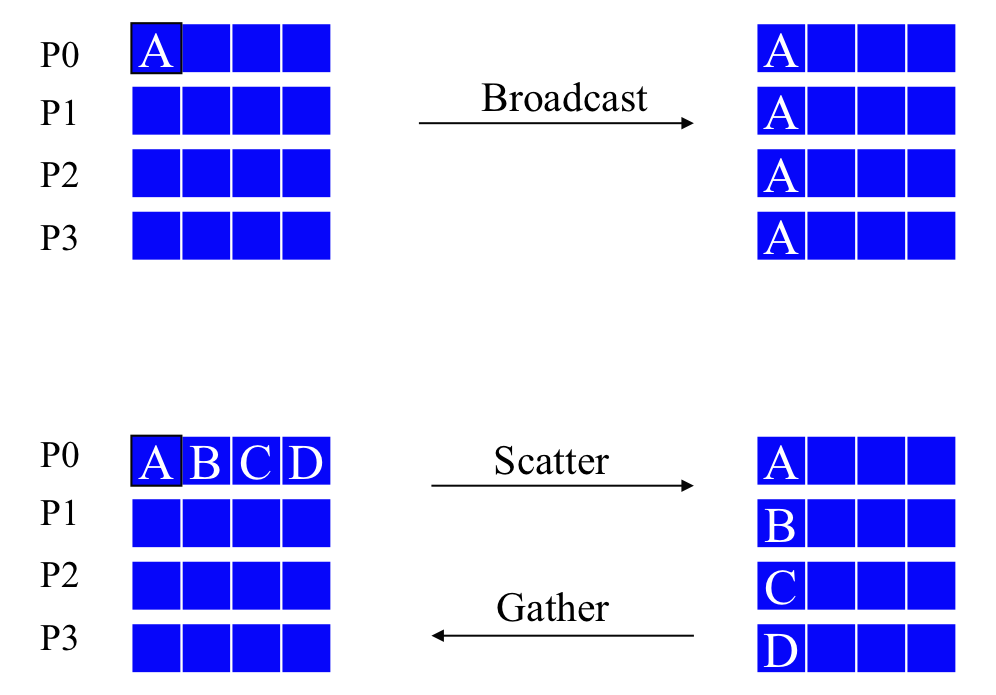
\includegraphics{../figures/broadcast_scatter_gather.png}
\end{figure}

    \paragraph{C}\label{c}

\begin{verbatim}
   int MPI_Bcast(void *buf, int count, MPI_Datatype type, 
   int root, MPI_Comm comm)
\end{verbatim}

\paragraph{mpi4py}\label{mpi4py}

\begin{verbatim}
  comm.Bcast(self, buf, root=0)
  comm.bcast(self, obj=None, root=0)
\end{verbatim}

    \subsection{Broadcast Example}\label{broadcast-example}

    \begin{Verbatim}[commandchars=\\\{\}]
{\color{incolor}In [{\color{incolor}54}]:} \PY{k}{if} \PY{n}{rank} \PY{o}{==} \PY{l+m+mi}{0}\PY{p}{:}
            \PY{n}{data} \PY{o}{=} \PY{p}{\PYZob{}}\PY{l+s}{\PYZsq{}}\PY{l+s}{key1}\PY{l+s}{\PYZsq{}} \PY{p}{:} \PY{p}{[}\PY{l+m+mi}{7}\PY{p}{,} \PY{l+m+mf}{2.72}\PY{p}{,} \PY{l+m+mi}{2}\PY{o}{+}\PY{l+m+mi}{3j}\PY{p}{]}\PY{p}{,}
                    \PY{l+s}{\PYZsq{}}\PY{l+s}{key2}\PY{l+s}{\PYZsq{}} \PY{p}{:} \PY{p}{(} \PY{l+s}{\PYZsq{}}\PY{l+s}{abc}\PY{l+s}{\PYZsq{}}\PY{p}{,} \PY{l+s}{\PYZsq{}}\PY{l+s}{xyz}\PY{l+s}{\PYZsq{}}\PY{p}{)}\PY{p}{\PYZcb{}}
         \PY{k}{else}\PY{p}{:}
            \PY{n}{data} \PY{o}{=} \PY{n+nb+bp}{None}
         \PY{n}{data} \PY{o}{=} \PY{n}{comm}\PY{o}{.}\PY{n}{bcast}\PY{p}{(}\PY{n}{data}\PY{p}{,} \PY{n}{root}\PY{o}{=}\PY{l+m+mi}{0}\PY{p}{)}
         \PY{k}{print} \PY{l+s}{\PYZdq{}}\PY{l+s}{bcast finished and data }\PY{l+s+se}{\PYZbs{}}
         \PY{l+s}{ on rank }\PY{l+s+si}{\PYZpc{}d}\PY{l+s}{ is: }\PY{l+s}{\PYZdq{}}\PY{o}{\PYZpc{}}\PY{k}{comm}\PY{o}{.}\PY{n}{rank}\PY{p}{,} \PY{n}{data}
\end{Verbatim}

    \begin{Verbatim}[commandchars=\\\{\}]
[stdout:0] bcast finished and data  on rank 0 is:  \{'key2': ('abc', 'xyz'), 'key1': [7, 2.72, (2+3j)]\}
[stdout:1] bcast finished and data  on rank 1 is:  \{'key2': ('abc', 'xyz'), 'key1': [7, 2.72, (2+3j)]\}
[stdout:2] bcast finished and data  on rank 3 is:  \{'key2': ('abc', 'xyz'), 'key1': [7, 2.72, (2+3j)]\}
[stdout:3] bcast finished and data  on rank 2 is:  \{'key2': ('abc', 'xyz'), 'key1': [7, 2.72, (2+3j)]\}
    \end{Verbatim}

    \subsection{Scatter Example:}\label{scatter-example}

    \begin{Verbatim}[commandchars=\\\{\}]
{\color{incolor}In [{\color{incolor}55}]:} \PY{k}{if} \PY{n}{rank} \PY{o}{==} \PY{l+m+mi}{0}\PY{p}{:}
            \PY{n}{data} \PY{o}{=} \PY{p}{[}\PY{p}{(}\PY{n}{i}\PY{o}{+}\PY{l+m+mi}{1}\PY{p}{)}\PY{o}{*}\PY{o}{*}\PY{l+m+mi}{2} \PY{k}{for} \PY{n}{i} \PY{o+ow}{in} \PY{n+nb}{range}\PY{p}{(}\PY{n}{size}\PY{p}{)}\PY{p}{]}
         \PY{k}{else}\PY{p}{:}
            \PY{n}{data} \PY{o}{=} \PY{n+nb+bp}{None}
         \PY{n}{data} \PY{o}{=} \PY{n}{comm}\PY{o}{.}\PY{n}{scatter}\PY{p}{(}\PY{n}{data}\PY{p}{,} \PY{n}{root}\PY{o}{=}\PY{l+m+mi}{0}\PY{p}{)}
         \PY{k}{assert} \PY{n}{data} \PY{o}{==} \PY{p}{(}\PY{n}{rank}\PY{o}{+}\PY{l+m+mi}{1}\PY{p}{)}\PY{o}{*}\PY{o}{*}\PY{l+m+mi}{2}
         \PY{k}{print} \PY{l+s}{\PYZdq{}}\PY{l+s}{data on rank }\PY{l+s+si}{\PYZpc{}d}\PY{l+s}{ is: }\PY{l+s}{\PYZdq{}}\PY{o}{\PYZpc{}}\PY{k}{comm}\PY{o}{.}\PY{n}{rank}\PY{p}{,} \PY{n}{data}
\end{Verbatim}

    \begin{Verbatim}[commandchars=\\\{\}]
[stdout:0] data on rank 0 is:  1
[stdout:1] data on rank 1 is:  4
[stdout:2] data on rank 3 is:  16
[stdout:3] data on rank 2 is:  9
    \end{Verbatim}

    \subsection{Gather (and Barrier)
Example:}\label{gather-and-barrier-example}

    \begin{Verbatim}[commandchars=\\\{\}]
{\color{incolor}In [{\color{incolor}56}]:} \PY{n}{data} \PY{o}{=} \PY{p}{(}\PY{n}{rank}\PY{o}{+}\PY{l+m+mi}{1}\PY{p}{)}\PY{o}{*}\PY{o}{*}\PY{l+m+mi}{2}
         \PY{k}{print} \PY{l+s}{\PYZdq{}}\PY{l+s}{before gather, data on }\PY{l+s+se}{\PYZbs{}}
         \PY{l+s}{  rank }\PY{l+s+si}{\PYZpc{}d}\PY{l+s}{ is: }\PY{l+s}{\PYZdq{}}\PY{o}{\PYZpc{}}\PY{k}{rank}\PY{p}{,} \PY{n}{data}
         
         \PY{n}{comm}\PY{o}{.}\PY{n}{Barrier}\PY{p}{(}\PY{p}{)}
         \PY{n}{data} \PY{o}{=} \PY{n}{comm}\PY{o}{.}\PY{n}{gather}\PY{p}{(}\PY{n}{data}\PY{p}{,} \PY{n}{root}\PY{o}{=}\PY{l+m+mi}{0}\PY{p}{)}
         \PY{k}{if} \PY{n}{rank} \PY{o}{==} \PY{l+m+mi}{0}\PY{p}{:}
            \PY{k}{for} \PY{n}{i} \PY{o+ow}{in} \PY{n+nb}{range}\PY{p}{(}\PY{n}{size}\PY{p}{)}\PY{p}{:}
                \PY{k}{assert} \PY{n}{data}\PY{p}{[}\PY{n}{i}\PY{p}{]} \PY{o}{==} \PY{p}{(}\PY{n}{i}\PY{o}{+}\PY{l+m+mi}{1}\PY{p}{)}\PY{o}{*}\PY{o}{*}\PY{l+m+mi}{2}
         \PY{k}{else}\PY{p}{:}
            \PY{k}{assert} \PY{n}{data} \PY{o+ow}{is} \PY{n+nb+bp}{None}
         \PY{k}{print} \PY{l+s}{\PYZdq{}}\PY{l+s}{data on rank: }\PY{l+s+si}{\PYZpc{}d}\PY{l+s}{ is: }\PY{l+s}{\PYZdq{}}\PY{o}{\PYZpc{}}\PY{k}{rank}\PY{p}{,} \PY{n}{data}
\end{Verbatim}

    \begin{Verbatim}[commandchars=\\\{\}]
[stdout:0] 
before gather, data on   rank 0 is:  1
data on rank: 0 is:  [1, 4, 9, 16]
[stdout:1] 
before gather, data on   rank 1 is:  4
data on rank: 1 is:  None
[stdout:2] 
before gather, data on   rank 3 is:  16
data on rank: 3 is:  None
[stdout:3] 
before gather, data on   rank 2 is:  9
data on rank: 2 is:  None
    \end{Verbatim}

    \subsection{Reduce and Scan}\label{reduce-and-scan}

\begin{figure}[htbp]
\centering
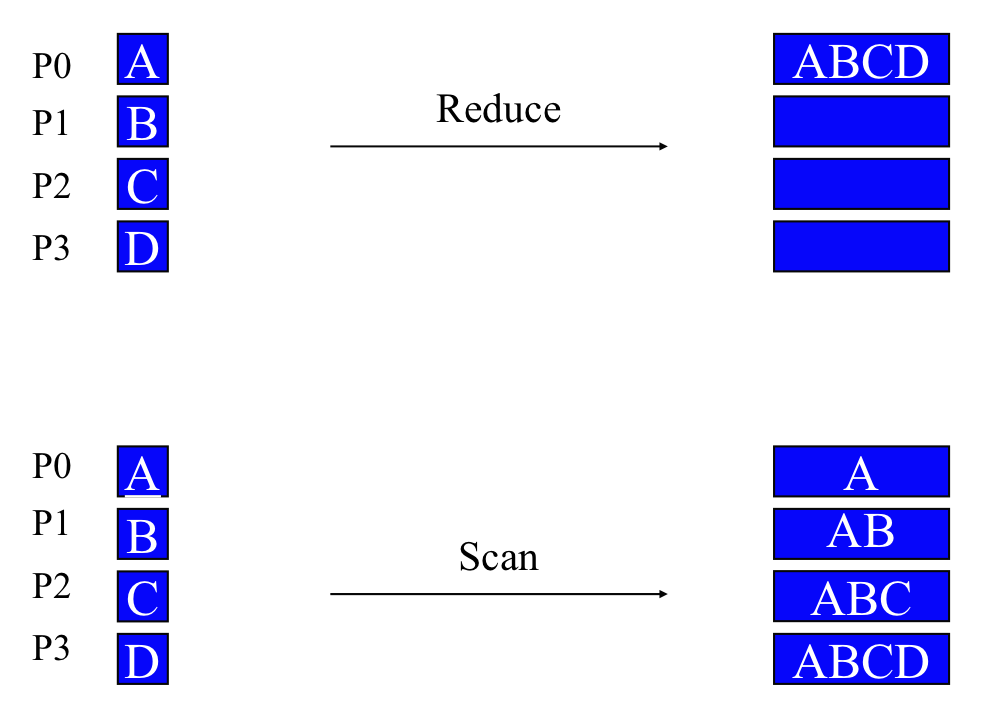
\includegraphics{../figures/reduce_scan.png}
\end{figure}

    \subsection{Reduce Example}\label{reduce-example}

The lower-case \texttt{reduce} implemented in \texttt{mpi4py} is not
designed to be particularly scalable. If you need to perform a reduce on
thousands of processes or more, it is recommended that you either switch
to the non-generic Reduce, or utilize the scalable reduce provided in
\texttt{mpi4py/demo/reductions/reductions.py}

    \begin{Verbatim}[commandchars=\\\{\}]
{\color{incolor}In [{\color{incolor}57}]:} \PY{n}{sendmsg} \PY{o}{=} \PY{n}{comm}\PY{o}{.}\PY{n}{rank}
         \PY{n}{recvmsg1} \PY{o}{=} \PY{n}{comm}\PY{o}{.}\PY{n}{reduce}\PY{p}{(}\PY{n}{sendmsg}\PY{p}{,} \PY{n}{op}\PY{o}{=}\PY{n}{MPI}\PY{o}{.}\PY{n}{SUM}\PY{p}{,} \PY{n}{root}\PY{o}{=}\PY{l+m+mi}{0}\PY{p}{)}
         \PY{n}{recvmsg2} \PY{o}{=} \PY{n}{comm}\PY{o}{.}\PY{n}{allreduce}\PY{p}{(}\PY{n}{sendmsg}\PY{p}{)}
         \PY{k}{print} \PY{n}{recvmsg2}
\end{Verbatim}

    \begin{Verbatim}[commandchars=\\\{\}]
[stdout:0] 6
[stdout:1] 6
[stdout:2] 6
[stdout:3] 6
    \end{Verbatim}

    \subsection{Compute Pi Example}\label{compute-pi-example}

The following example is completely self-contained to simplify reuse in
another script. You can switch between running the code in parallel and
serial by executing an \%autopx cell.

    \begin{Verbatim}[commandchars=\\\{\}]
{\color{incolor}In [{\color{incolor}33}]:} \PY{k+kn}{from} \PY{n+nn}{mpi4py} \PY{k+kn}{import} \PY{n}{MPI}
         \PY{k+kn}{import} \PY{n+nn}{math}
         
         \PY{k}{def} \PY{n+nf}{compute\PYZus{}pi}\PY{p}{(}\PY{n}{n}\PY{p}{,} \PY{n}{start}\PY{o}{=}\PY{l+m+mi}{0}\PY{p}{,} \PY{n}{step}\PY{o}{=}\PY{l+m+mi}{1}\PY{p}{)}\PY{p}{:}
             \PY{n}{h} \PY{o}{=} \PY{l+m+mf}{1.0} \PY{o}{/} \PY{n}{n}
             \PY{n}{s} \PY{o}{=} \PY{l+m+mf}{0.0}
             \PY{k}{for} \PY{n}{i} \PY{o+ow}{in} \PY{n+nb}{range}\PY{p}{(}\PY{n}{start}\PY{p}{,} \PY{n}{n}\PY{p}{,} \PY{n}{step}\PY{p}{)}\PY{p}{:}
                 \PY{n}{x} \PY{o}{=} \PY{n}{h} \PY{o}{*} \PY{p}{(}\PY{n}{i} \PY{o}{+} \PY{l+m+mf}{0.5}\PY{p}{)}
                 \PY{n}{s} \PY{o}{+}\PY{o}{=} \PY{l+m+mf}{4.0} \PY{o}{/} \PY{p}{(}\PY{l+m+mf}{1.0} \PY{o}{+} \PY{n}{x}\PY{o}{*}\PY{o}{*}\PY{l+m+mi}{2}\PY{p}{)}
             \PY{k}{return} \PY{n}{s} \PY{o}{*} \PY{n}{h}
         
         \PY{n}{comm} \PY{o}{=} \PY{n}{MPI}\PY{o}{.}\PY{n}{COMM\PYZus{}WORLD}
         \PY{n}{nprocs} \PY{o}{=} \PY{n}{comm}\PY{o}{.}\PY{n}{Get\PYZus{}size}\PY{p}{(}\PY{p}{)}
         \PY{n}{myrank} \PY{o}{=} \PY{n}{comm}\PY{o}{.}\PY{n}{Get\PYZus{}rank}\PY{p}{(}\PY{p}{)}
         \PY{k}{if} \PY{n}{myrank} \PY{o}{==} \PY{l+m+mi}{0}\PY{p}{:}
             \PY{n}{n} \PY{o}{=} \PY{l+m+mi}{10}
         \PY{k}{else}\PY{p}{:}
             \PY{n}{n} \PY{o}{=} \PY{n+nb+bp}{None}
         
         \PY{n}{n} \PY{o}{=} \PY{n}{comm}\PY{o}{.}\PY{n}{bcast}\PY{p}{(}\PY{n}{n}\PY{p}{,} \PY{n}{root}\PY{o}{=}\PY{l+m+mi}{0}\PY{p}{)}
         
         \PY{n}{mypi} \PY{o}{=} \PY{n}{compute\PYZus{}pi}\PY{p}{(}\PY{n}{n}\PY{p}{,} \PY{n}{myrank}\PY{p}{,} \PY{n}{nprocs}\PY{p}{)}
         
         \PY{n}{pi} \PY{o}{=} \PY{n}{comm}\PY{o}{.}\PY{n}{reduce}\PY{p}{(}\PY{n}{mypi}\PY{p}{,} \PY{n}{op}\PY{o}{=}\PY{n}{MPI}\PY{o}{.}\PY{n}{SUM}\PY{p}{,} \PY{n}{root}\PY{o}{=}\PY{l+m+mi}{0}\PY{p}{)}
         
         \PY{k}{if} \PY{n}{myrank} \PY{o}{==} \PY{l+m+mi}{0}\PY{p}{:}
             \PY{n}{error} \PY{o}{=} \PY{n+nb}{abs}\PY{p}{(}\PY{n}{pi} \PY{o}{\PYZhy{}} \PY{n}{math}\PY{o}{.}\PY{n}{pi}\PY{p}{)}
             \PY{k}{print} \PY{p}{(}\PY{l+s}{\PYZdq{}}\PY{l+s}{pi is approximately }\PY{l+s+si}{\PYZpc{}.16f}\PY{l+s+se}{\PYZbs{}n}\PY{l+s}{error is }\PY{l+s+si}{\PYZpc{}.16f}\PY{l+s}{\PYZdq{}} \PY{o}{\PYZpc{}} \PY{p}{(}\PY{n}{pi}\PY{p}{,} \PY{n}{error}\PY{p}{)}\PY{p}{)}
\end{Verbatim}

    \begin{Verbatim}[commandchars=\\\{\}]
[stdout:3] 
pi is approximately 3.1424259850010983
error is 0.0008333314113051
    \end{Verbatim}

    \subsection{Mandelbrot Set Example}\label{mandelbrot-set-example}

The following example is completely self-contained to simplify reuse in
another script.

    \begin{Verbatim}[commandchars=\\\{\}]
{\color{incolor}In [{\color{incolor}41}]:} \PY{k+kn}{from} \PY{n+nn}{mpi4py} \PY{k+kn}{import} \PY{n}{MPI}
         \PY{k+kn}{import} \PY{n+nn}{numpy} \PY{k+kn}{as} \PY{n+nn}{np}
         
         \PY{k}{def} \PY{n+nf}{mandelbrot} \PY{p}{(}\PY{n}{x}\PY{p}{,} \PY{n}{y}\PY{p}{,} \PY{n}{maxit}\PY{p}{)}\PY{p}{:}
             \PY{n}{c} \PY{o}{=} \PY{n}{x} \PY{o}{+} \PY{n}{y}\PY{o}{*}\PY{l+m+mi}{1j}
             \PY{n}{z} \PY{o}{=} \PY{l+m+mi}{0} \PY{o}{+} \PY{l+m+mi}{0j}
             \PY{n}{it} \PY{o}{=} \PY{l+m+mi}{0}
             \PY{k}{while} \PY{n+nb}{abs}\PY{p}{(}\PY{n}{z}\PY{p}{)} \PY{o}{\PYZlt{}} \PY{l+m+mi}{2} \PY{o+ow}{and} \PY{n}{it} \PY{o}{\PYZlt{}} \PY{n}{maxit}\PY{p}{:}
                 \PY{n}{z} \PY{o}{=} \PY{n}{z}\PY{o}{*}\PY{o}{*}\PY{l+m+mi}{2} \PY{o}{+} \PY{n}{c}
                 \PY{n}{it} \PY{o}{+}\PY{o}{=} \PY{l+m+mi}{1}
             \PY{k}{return} \PY{n}{it}
         
         \PY{n}{x1}\PY{p}{,} \PY{n}{x2} \PY{o}{=} \PY{o}{\PYZhy{}}\PY{l+m+mf}{2.0}\PY{p}{,} \PY{l+m+mf}{1.0}
         \PY{n}{y1}\PY{p}{,} \PY{n}{y2} \PY{o}{=} \PY{o}{\PYZhy{}}\PY{l+m+mf}{1.0}\PY{p}{,} \PY{l+m+mf}{1.0}
         \PY{n}{w}\PY{p}{,} \PY{n}{h} \PY{o}{=} \PY{l+m+mi}{250}\PY{p}{,} \PY{l+m+mi}{200}
         \PY{n}{maxit} \PY{o}{=} \PY{l+m+mi}{127}
           
         \PY{n}{comm} \PY{o}{=} \PY{n}{MPI}\PY{o}{.}\PY{n}{COMM\PYZus{}WORLD}
         \PY{n}{size} \PY{o}{=} \PY{n}{comm}\PY{o}{.}\PY{n}{Get\PYZus{}size}\PY{p}{(}\PY{p}{)}
         \PY{n}{rank} \PY{o}{=} \PY{n}{comm}\PY{o}{.}\PY{n}{Get\PYZus{}rank}\PY{p}{(}\PY{p}{)}
         
         \PY{c}{\PYZsh{} number of rows to compute here}
         \PY{n}{N} \PY{o}{=} \PY{n}{h} \PY{o}{/}\PY{o}{/} \PY{n}{size} \PY{o}{+} \PY{p}{(}\PY{n}{h} \PY{o}{\PYZpc{}} \PY{n}{size} \PY{o}{\PYZgt{}} \PY{n}{rank}\PY{p}{)}
         
         \PY{c}{\PYZsh{} first row to compute here}
         \PY{n}{start} \PY{o}{=} \PY{n}{comm}\PY{o}{.}\PY{n}{scan}\PY{p}{(}\PY{n}{N}\PY{p}{)}\PY{o}{\PYZhy{}}\PY{n}{N}
         
         \PY{c}{\PYZsh{} array to store local result}
         \PY{n}{Cl} \PY{o}{=} \PY{n}{np}\PY{o}{.}\PY{n}{zeros}\PY{p}{(}\PY{p}{[}\PY{n}{N}\PY{p}{,} \PY{n}{w}\PY{p}{]}\PY{p}{,} \PY{n}{dtype}\PY{o}{=}\PY{l+s}{\PYZsq{}}\PY{l+s}{i}\PY{l+s}{\PYZsq{}}\PY{p}{)}
         
         \PY{c}{\PYZsh{} compute owned rows}
         
         \PY{n}{dx} \PY{o}{=} \PY{p}{(}\PY{n}{x2} \PY{o}{\PYZhy{}} \PY{n}{x1}\PY{p}{)} \PY{o}{/} \PY{n}{w}
         \PY{n}{dy} \PY{o}{=} \PY{p}{(}\PY{n}{y2} \PY{o}{\PYZhy{}} \PY{n}{y1}\PY{p}{)} \PY{o}{/} \PY{n}{h}
         
         \PY{k}{for} \PY{n}{i} \PY{o+ow}{in} \PY{n+nb}{range}\PY{p}{(}\PY{n}{N}\PY{p}{)}\PY{p}{:}
             \PY{n}{y} \PY{o}{=} \PY{n}{y1} \PY{o}{+} \PY{p}{(}\PY{n}{i} \PY{o}{+} \PY{n}{start}\PY{p}{)} \PY{o}{*} \PY{n}{dy}
             \PY{k}{for} \PY{n}{j} \PY{o+ow}{in} \PY{n+nb}{range}\PY{p}{(}\PY{n}{w}\PY{p}{)}\PY{p}{:}
                 \PY{n}{x} \PY{o}{=} \PY{n}{x1} \PY{o}{+} \PY{n}{j} \PY{o}{*} \PY{n}{dx}
                 \PY{n}{Cl}\PY{p}{[}\PY{n}{i}\PY{p}{,} \PY{n}{j}\PY{p}{]} \PY{o}{=} \PY{n}{mandelbrot}\PY{p}{(}\PY{n}{x}\PY{p}{,} \PY{n}{y}\PY{p}{,} \PY{n}{maxit}\PY{p}{)}
         
         \PY{c}{\PYZsh{} gather results at root (process 0)}
         \PY{n}{counts} \PY{o}{=} \PY{n}{comm}\PY{o}{.}\PY{n}{gather}\PY{p}{(}\PY{n}{N}\PY{p}{,} \PY{n}{root}\PY{o}{=}\PY{l+m+mi}{0}\PY{p}{)}
         \PY{n}{C} \PY{o}{=} \PY{n+nb+bp}{None}
         \PY{k}{if} \PY{n}{rank} \PY{o}{==} \PY{l+m+mi}{0}\PY{p}{:}
             \PY{n}{C} \PY{o}{=} \PY{n}{np}\PY{o}{.}\PY{n}{zeros}\PY{p}{(}\PY{p}{[}\PY{n}{h}\PY{p}{,} \PY{n}{w}\PY{p}{]}\PY{p}{,} \PY{n}{dtype}\PY{o}{=}\PY{l+s}{\PYZsq{}}\PY{l+s}{i}\PY{l+s}{\PYZsq{}}\PY{p}{)}
         
         \PY{c}{\PYZsh{} here we create a custom datatype for sending/receiving rows of data.}
         \PY{n}{rowtype} \PY{o}{=} \PY{n}{MPI}\PY{o}{.}\PY{n}{INT}\PY{o}{.}\PY{n}{Create\PYZus{}contiguous}\PY{p}{(}\PY{n}{w}\PY{p}{)}
         \PY{n}{rowtype}\PY{o}{.}\PY{n}{Commit}\PY{p}{(}\PY{p}{)}
         
         \PY{n}{comm}\PY{o}{.}\PY{n}{Gatherv}\PY{p}{(}\PY{n}{sendbuf}\PY{o}{=}\PY{p}{[}\PY{n}{Cl}\PY{p}{,} \PY{n}{MPI}\PY{o}{.}\PY{n}{INT}\PY{p}{]}\PY{p}{,} \PY{n}{recvbuf}\PY{o}{=}\PY{p}{[}\PY{n}{C}\PY{p}{,} \PY{p}{(}\PY{n}{counts}\PY{p}{,} \PY{n+nb+bp}{None}\PY{p}{)}\PY{p}{,} \PY{n}{rowtype}\PY{p}{]}\PY{p}{,}\PY{n}{root}\PY{o}{=}\PY{l+m+mi}{0}\PY{p}{)}
         
         \PY{n}{rowtype}\PY{o}{.}\PY{n}{Free}\PY{p}{(}\PY{p}{)}
\end{Verbatim}

    We can't inline plots from the \texttt{ipcluster} Engines where we just
performed the computations. Instead, we use the Notebook Engine to get a
copy of the data on MPI rank 0, then plot as before.

First, we switch off \texttt{\%autopx} to enable computing on the
Notebook Engine.

    \begin{Verbatim}[commandchars=\\\{\}]
{\color{incolor}In [{\color{incolor}42}]:} \PY{o}{\PYZpc{}}\PY{k}{autopx}
\end{Verbatim}

    \begin{Verbatim}[commandchars=\\\{\}]
\%autopx disabled
    \end{Verbatim}

    Then we collect the array and rank data from the \texttt{ipcluster}
Engines using the \texttt{view} object.

    \begin{Verbatim}[commandchars=\\\{\}]
{\color{incolor}In [{\color{incolor}43}]:} \PY{c}{\PYZsh{} CC is a list of C from all ranks}
         \PY{n}{CC} \PY{o}{=} \PY{n}{view}\PY{p}{[}\PY{l+s}{\PYZsq{}}\PY{l+s}{C}\PY{l+s}{\PYZsq{}}\PY{p}{]}
         \PY{c}{\PYZsh{} Similarly, ranks is a list of MPI ranks from all ipcluster processes}
         \PY{n}{ranks} \PY{o}{=} \PY{n}{view}\PY{p}{[}\PY{l+s}{\PYZsq{}}\PY{l+s}{rank}\PY{l+s}{\PYZsq{}}\PY{p}{]}
         
         \PY{c}{\PYZsh{} Do the plotting}
         \PY{c}{\PYZsh{} We use the IPython index of the ipcluster process with rank 0 as}
         \PY{c}{\PYZsh{} the index into CC}
         \PY{n}{pyplot}\PY{o}{.}\PY{n}{imshow}\PY{p}{(}\PY{n}{CC}\PY{p}{[}\PY{n}{ranks}\PY{o}{.}\PY{n}{index}\PY{p}{(}\PY{l+m+mi}{0}\PY{p}{)}\PY{p}{]}\PY{p}{)}
         \PY{n}{pyplot}\PY{o}{.}\PY{n}{spectral}\PY{p}{(}\PY{p}{)}
         \PY{n}{pyplot}\PY{o}{.}\PY{n}{show}\PY{p}{(}\PY{p}{)}
\end{Verbatim}

    \begin{center}
    \adjustimage{max size={0.9\linewidth}{0.9\paperheight}}{03.1_Distributed_Computing_files/03.1_Distributed_Computing_65_0.png}
    \end{center}
    { \hspace*{\fill} \\}
    

    % Add a bibliography block to the postdoc
    
    
    
    \end{document}
